\documentclass[10pt,journal]{IEEEtran}

\usepackage{graphicx}

\usepackage{silence}
\WarningFilter{biblatex}{File 'english-ieee.lbx'}

\DeclareFixedFont{\ttb}{T1}{txtt}{bx}{n}{5} % for bold
\DeclareFixedFont{\ttm}{T1}{txtt}{m}{n}{5}  % for normal

% Custom colors
\usepackage{xcolor}
\definecolor{deepblue}{rgb}{0,0,0.5}
\definecolor{deepred}{rgb}{0.6,0,0}
\definecolor{deepgreen}{rgb}{0,0.5,0}

\usepackage{listings}

% Python style for highlighting
\newcommand\pythonstyle{\lstset{
language=Python,
basicstyle=\ttm,
otherkeywords={self},             % Add keywords here
keywordstyle=\ttb\color{deepblue},
emph={SinKew,__init__},          % Custom highlighting
emphstyle=\ttb\color{deepred},    % Custom highlighting style
stringstyle=\color{deepgreen},
frame=tb,                         % Any extra options here
numbers=left,
stepnumber=5,
showstringspaces=false            % 
framexleftmargin=25px
}}

\newcommand\pythonexternal[2][]{{
\pythonstyle
\lstinputlisting[#1]{#2}}}

% ------- set darkmode -----------
%\usepackage{xcolor}
%\pagecolor[rgb]{0.2,0.2,0.2}
%\color[rgb]{1,1,1}
% --------------------------------

\usepackage{lipsum}

\usepackage[style=authoryear-ibid, backend=biber]{biblatex}
\addbibresource{report.bib}

%\bibliographystyle{IEEEtran}
%\bibliography{IEEEabrv,report.bib}

\title{\textbf{RESEARCHING THE ABILITY OF REINFORCEMENT LEARNING AGENTS TO ADAPT TO CHANGES IN THEIR TRAINING ENVIRONMENT}\\}

%\title{\textbf{Developing Flexible Reinforcement Learning Environments to Understand Their Effect on the Trained Agent}\\}

\author{Tomos Ody (ODY14527411)\\Department of Computer Science, University of Lincoln}

\date{29th August 2019}

\begin{document}

\maketitle

\begin{abstract}
  The quick brown fox jumped over the lazy dog \lipsum[1]
\end{abstract}

\section{Introduction}

\subsection{Rationale}
Much of the Reinforcement Learning \textbf{(RL)} literature is focused around specific best case applications to specific problem domains. This is an improvement over past trends described in Kaelbling's survey of the subject from 1996 \cite{Kaelbling} where research was being done on poorly defined problem domains. More recently RL research has become more focused into complex and specific problem domains. However there is little research comparing the various RL methods to one another in a comprehensive manner. Often with brief discussions of the various methods without evidence validating the chosen RL methodology. More often than not the choice of method comes down to examination of the problem domain to be explored.

The focus of this project is in comparing the performance of the more popular Q-Learning \textbf{(QL)}  control policy (\cite{Watkins92}) against the lesser known State-Action-Reward-State-Action \textbf{(SARSA)} control policy (\cite{Rummery}) in as comprehensive a manner as possible. With the aim of understanding how applicable these methods are to various problem domains and situations. In theory SARSA should always outperform QL since it always evaluates it’s chosen action (\cite{Sutton}). And is the more computationally expensive method as a result.

Q-Learning and SARSA are very closely related temporal difference \textbf{(TD)} problems and so many optimizations of one are applicable to the other. This makes them simple to compare against one another as well as understand the differences in reinforcement learning environments. However QL overshadows SARSA in the literature quite dramatically, to the point SARSA is considerably harder to research than QL in the academic literature, however I have been unable to find an obvious reason why.

\subsection{Aims and Objectives}
The aim of this project is to understand the differences in performance of QL and SARSA and by extension offline and online control policies for TD problems. With focus being drawn to how the environments used for training affect the performance of the various control policies.

Further research will be conducted to understand the scope of TD problem domains as well as explore potential optimisations of QL and SARSA. This will allow the analysis to be more complete and present additional opportunities for comparison between the control policies.

The reason for the prevalence of QL over SARSA in the academic literature should be explored. Experimental data will be considered alongside the literature to inform the evaluation of these control policies for TD problems.

\subsection{Hypothesis}

\subsection{Background}

\subsubsection{Reinforcement Learning}
RL is distinct from most Artificial Intelligence \textbf{(AI)} disciplines in that instead of relying on a large pool of ground truth examples for the learning to be done upon. Instead RL relies on the design of the learning environment to teach an AI how to perform a task. In most cases this is done through reward functions with the RL agent inferring from these rewards how the task should be performed (\cite{Kaelbling}).

This however relies on the designed learning environment being simple enough for an agent to learn from it’s interactions with the environment alone. This leads to the main challenge in RL, exploration vs exploitation. This describes the balance between the agent exploring the environment to update all actions with their corresponding rewards and exploiting the already learned actions, taking the optimal action. This is important as it not only decides how the agent learns the environment but also its ability to interact with the environment effectively. Since if the agent always takes random actions to explore the environment fully it will never learn the optimal strategy. Likewise if the agent only follows the optimal strategy it will not learn better strategies if they exist. This can drastically affect the time it takes to train the agent since being too close to one extreme or the other causes the agent to either never learn the optimal strategy or learn an incorrect optimal strategy by never encountering the optimal strategy (\cite{Sutton}).

\subsubsection{Q-Learning}
Q-Learning was initially proposed by Watkins in their Phd thesis \cite{Watkins89} building on MDPs to solve more complex problems without the difficulty of building an equally complex model to solve it. Q-Learning was formalised 3 years later in \cite{Watkins92}.

“It provides  agents with the capability of learning to act optimally in Markovian domains by experiencing the con-sequences of actions, without requiring them to build maps of the domains.” (\cite[55]{Watkins92})

Q-Learning simplifies the environment into a Q-table with the dimensions $$[number \: of \: states, \; number \: of \: actions]$$ Each point in the table corresponds to a Q-value for an action at the given state. This table allows for the agent to learn from the experience of each state and action. By following the maximum Q-value the optimal path should be followed given that all Q-values are representative of the environment. However, the discrete nature of the Q-table means that QL is limited to discrete problems or the environment must be discretized leading to a loss in state and action accuracy (\cite{Gaskett}). 

\subsubsection{SARSA}

\subsubsection{Temporal Difference Learning}

\subsection{Report Structure}

\tableofcontents{}

\section{Literature Review}

\subsection{Academic basis}
The standard RL model consists of an agent interacting with an environment via perception and action. At each step of the training process the agent receives some state information. Based on this information the agent will then take an action based on it's observations of the environment. Depending on the action taken a scalar reinforcement signal is sent to the agent as a reflection of success. The agent aims to maximise the long-run sum of the reinforcement signal. This process leads to the agent choosing the rewarded actions leading to the development of the desired behaviour in the agent. As outlined in \cite{Kaelbling}, a survey of RL field from 1996. This basic outline is corroborated by \cite{Busoniu}, a survey of multiagent RL from 2008 and \cite{Kober}, a survey of RL in robotics from 2013. This basic conception of RL models is consistent across all literature and appears in papers up to the current day.

This learning method does not fit neatly into the two main machine learning paradigms of supervised and unsupervised learning. Instead of being directly trained by correct examples or inferring patterns from the data, a RL agent learns from it's own interactions with the environment quantified by a scalar reward described in the book Reinforcement Learning: An Introduction \cite{Sutton}, cited in many RL works. This agent driven learning style leads to a trade-off between exploration and exploitation (\cite{Sutton, Kaelbling, Busoniu, Kober}). Due to the need for the agent to explore the environment as well as perform actions to maximise the positive reward (exploitation). The trade-off stems from the incompatibility of these two behaviours which are both required for an effective agent. Since the agent must explore the environment to understand the positive and negative options possible yet avoid negative actions to succeed (\cite{Kaelbling}). For most RL problems Markov Decision Processes (MDP) are applied as the methodology for modelling decisions to calculate action rewards accounting for the exploration-exploitation trade-off (\cite{Kober}). MDPs work by considering rewards temporally, meaning that a series of actions can be attributed to the delayed reward function (\cite{Kaelbling, Busoniu, Kober}). This is in contrast to more simple greedy strategies which reward the agent directly for each individual action. However these methods can fall victim to unlucky reward sampling early in the training process (\cite{Kaelbling}). A useful framing problem for understanding the balancing of exploration and exploitation is the K-Armed Bandit problem. This is used in most survey papers (\cite{Kaelbling, Busoniu, Kober}) to explore the performance of RL methods in the scope of exploration vs exploitation. The more recent papers \cite{Busoniu, Kober} analysing these methods to balance exploration and exploitation tend towards the more dynamic methods like MDPs as opposed to the more simplistic greedy strategies mentioned in \cite{Kaelbling}. The other simplistic methods suggested by \cite{Kaelbling} are not mentioned in the more recent surveys of RL \cite{Busoniu, Kober}, only in \cite{Sutton} are these methods mentioned as introductory methods to RL. The literature seems to be in agreement on many of the details of RL methods, however many methods mentioned in the older \cite{Kaelbling} seem to be less widely used in the surveys written in recent years (\cite{Busoniu, Kober}).

Most of the methods discussed in RL are very old, for example MDPs were originally proposed by \cite{Bellman} in 1958 which is cited in each of the RL surveys \cite{Kaelbling, Busoniu, Kober} as well as the seminal \cite{Sutton}. The vast majority of improvements made to RL methods are minor improvements to MDPs.

\subsection{Scope of reinforcement learning}
Reinforcement learning is a very adaptable machine learning approach due to the wide range of approaches and methodologies that can be used to form a solution. However \cite{Kaelbling} concludes that RL performs well on small problems but poorly on larger problems due to the efficiency of generalising the problems. This point is reaffirmed by \cite{Wirth}, adding that an efficient generalisation of a complex problem requires expert domain knowledge. This suggests that whilst versatile, RL is only generally suited to simple problems.

One of the primary areas of RL research is robotics since the domain of controlling a robot fits neatly into a RL problem as discussed in \cite{Kober}, whereas other machine learning disciplines are very difficult to utilise for robotic control systems. This view of RL in robotics is shared by \cite{Smart}. Many other hurdles are introduced by using reinforcement learning in a real context such as observation inaccuracies and the expense of hardware \cite{Kober}, however this does not pertain to this project. Robotic RL agents instead present a strong base of real agent-environment interactions (\cite{Kober}).

Up till this point single-agent systems have been discussed, however Multi-Agent Reinforcement Learning (MARL) is another large body of work with multiple agents training in the same environment. This domain is similar to single-agent RL but multiple agents open up a new set of challenges and advantages. As described in \cite{Busoniu} the main challenge faced is an exacerbation of the exploration-exploitation trade-off due to inter-agent interactions adding a new level of complexity to the issue. Multiple agents can also be turned into an advantage in MARL by allowing agents to share their experience with other agents. Additionally more advanced reward functions can encourage collaborative actions between agents. One clear advantage over other RL domains is that MARL can benefit from parallel computing increasing the computational efficiency.

Most RL environments could be described as games, unsurprisingly the most active domain of RL is playing video games. Video games present a host of environments easily adaptable to RL applications, however the low complexity tolerance of RL still takes effect. This leads to either very simplistic games being used to train complete agents to perform well such as in \cite{Bellemare} or more high level applications like \cite{Amato} where a RL agent controls the strategies of an artificial intelligence agent designed to play the game. These applications both use MDPs with Q-Leaning (\cite{Watkins92}) to consider the higher level temporal planning required for playing video games.

A criticism is raised in \cite{Shoham}, a critical survey of MARL using MDPs, as to the definition of many RL solutions in that they are often performed from an ill defined domain basis in how learning best occurs. It outlines a four stage method of properly defining a RL problem, describing how too many RL solutions work off previous bases without exploring their applicability to the problem being addressed. 
% reconsider Ng as a citation due to multiple versions and springer being shit
This demonstrated by the contrast between \cite{Amato} where little academically supported domain knowledge is presented versus \cite{Ng} where the domain knowledge is comprehensively explored before designing the RL solution. This suggests that certain areas of RL problems are ill guided.

\subsection{Reinforcement learning techniques}
Whilst not encompassing all of RL, MDPs represent the vast majority of modern machine learning solutions. This is due to the simplicity with which a complex problem can be represented, taking into account time and previous actions as outlined in \cite{Barto}. As a result of this focus there is a wealth of different MDP strategies in the literature to draw from. An MDP is a framework for modelling actions with controllable yet undetermined outcomes to be optimised \cite{Bellman}. Utilising an MDP a complex problem can be abstracted down to a comparably computationally simple problem, this however requires much domain specific knowledge to be properly exercised \cite{Shoham}.

MDPs are a mathematical framework to quantify and rationalise decisions made in a Stochastic Game (SG) \cite{Bellman}. SGs are step by step games which quantify an environment probabilistically \cite{Shapley}, this hugely simplifies reward and action computation in RL problems \cite{Busoniu}.

In both \cite{Bellemare, Amato} Q-Learning is used, it is an approach to MDPs which allows a RL agent to explore an environment to experience the various reward states associated with each action. The Q-Learning task will use these immediate rewards to plan temporally how to maximise the reward overall as described in \cite{Watkins92}. 

Much of the research pertaining to RL problems seems much too condensed, with single authors appearing in multiple papers such as Barto in \cite{Barto} as well as the book \cite{Sutton}. Kaelbling also appears in both \cite{Kaelbling, Smart}. Other concentrations like this appear all across the RL literature which makes me sceptical of the academic basis of many of these methodologies. 

\section{Methodology}

\section{Design and Development}

\section{Experiments and Evaluation}

\begin{figure}
  \caption{oho it's a huge graph}
  \centering
  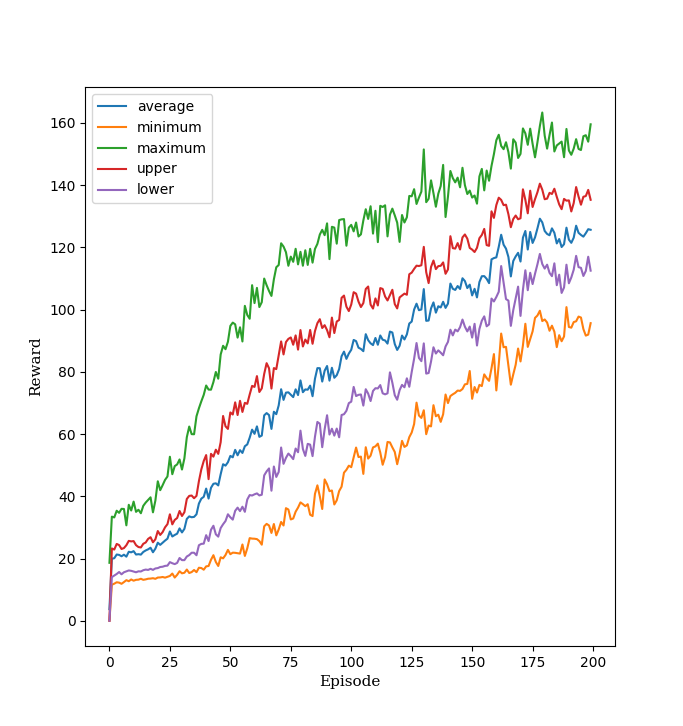
\includegraphics[width=0.5\textwidth]{Figure_1.png}
\end{figure}

\begin{figure}
  \caption{this is much more manageable}
  \centering
  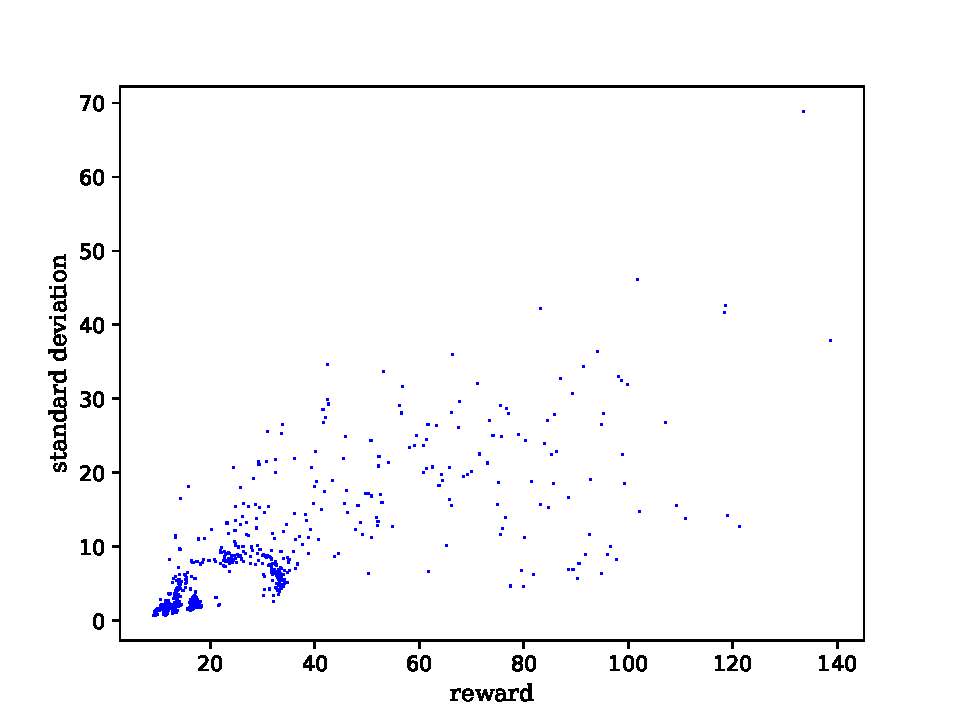
\includegraphics[scale=0.5]{Figure_2.pdf}
\end{figure}

\section{Discussions and Reflective Analysis}

\section{Conclusion}

\addcontentsline{toc}{section}{References}
\setlength\bibitemsep{1.7\itemsep plus 1pt minus 1pt}
\printbibliography

\appendix

\scriptsize
\pythonexternal{final.py}[linewidth=5.4]

\addcontentsline{toc}{section}{Acknowledgements}
\section*{Acknowledgements}

\end{document}
